\documentclass[12pt]{report}
\usepackage{graphicx}
\usepackage{natbib}
\usepackage{tabu}

\title{Thesis}
\author{Kilian Callebaut}

\begin{document}
	
	% include table of which combinations to compare
	% clearer in what kind of framework to plug
	% specify the combinations of what you're comparing
	% what are the most critical questions
	% strip complexity of the test
	% Clarity on measures you are actually using
	% resource efficiency
	% really only on the predictive power
	
	\maketitle
	
	\tableofcontents
	
	% Research gap fix
	\chapter{Introduction}

\section{Context}
% Don't start about lifelogging
% Start about Multi-Task learning, Audio classification and the gap in those fields

An important aspect to a lot of technological developments has always been the support and augmentation of human bodily functions, from developing hearing aids to improve auditory perception to robotic exoskeletons for supporting human movement. One such functions is human memory, the augmentation of which is targeted by developing life logging technology. Typically memory aids come in the form of photographs, notes or diaries, but all of these require planning and physical effort which may not be possible or fast enough at all times. Lifelogging however, can counter these shortcomings and help mitigate memory lapses. According to \citet{harvey2016remembering}, lifelogging is a "form of pervasive computing, consisting of a unified digital record of the totality of an individuals experiences, captured multi-modally through digital sensors and stored permanently as a personal multimedia archive". Lifelogging, in other words, is a digital diary of events and environments, stored not only for the aid, but the augmentation of human memory by means of retrieval and representation of data recorded by cameras and wearable sensors \cite{harvey2016remembering}.\\

Lifelogging also has capabilities outside of memory related functionalities. According to \citet{tzelepis2016event}, the goal of lifelogging is analyzing bahavior and experiences in terms of events, states and relationships. This reveals a more digital surveillance side, which has seen applications in health monitoring \cite{hamid2017survey}, workplace safety \cite{lee2020evidence} and personal recommendation systems \cite{yamano2009browsing}. It can help us analyze what is happening during a day and find and track correlations we might not have been able to perform ourselves, on a personal basis as well as on a group basis. A challenging problem to this however is recognizing specific events and environments after identifying the boundaries first \cite{tzelepis2016event}. This is necessary for efficient semantically annotating of captured data for later retrieval and/or analysis.\\

While there are some systems that only focus on lifelogging through audio (Kapture, Vemuri,S., S. Chris. \& B. Walter. iRemember: a Personal, Long-term Memory Prosthesis. 3rd ACM Workshop on Continous Archival and Retrieval of Persoanl Experiences CARPE' 06: 65-74 (2006)., ) \cite{shah2012lifelogging}, it has largely been disregarded. Sources for lifelogs mostly come from images, video, GPS and Physiological data (e.g. step counters), with audio sources being seen as more contested, additional information to those \cite{harvey2016remembering}. However, as \citet{yamano2009browsing} point out, audio from speech can provide information on conversations and ambient background noise can identify the environment and its characteristics better than only using previous sources. Audio sensors also offer the benefits of easy deployment, omnidirectional coverage and specular reflections of the signal can be used as a form of audio input (e.g. to derive the spaciousness of the room) \cite{chandrakala2019environmental}. This demonstrates how audio can improve context and event recognition capabilities for building a lifelog of events during the day. \\

The primary functions of a sensor based lifelogging system are described by \citet{ali2019insight} as "determining a set of target events and associating sensory data and other inputs as contexts to the events". Determining both the type as well as the beginning and end time of acoustic activity events is referred to Acoustic Event Detection (AED) and has seen a growing interest from the scientific community. While conventional pattern recognition methods like SVM's, GMM's and HMM's have been applied for this task, they have fallen short when audio events are overlapping or when strong labels (both the type of event and the temporal boundaries) are not available \cite{xia2019survey}. In real life audio recordings, events are often overlapping . Neural Network-based deep learning approaches have tried to address these problems in AED. Neural network methods adopted for AED include Deep Neural Networks (DNN) (CITE), Recurrent Neural Networks (RNN) (CITE), Convolutional Neural Networks (CNN) (CITE) and Convolutional Recurrent Neural Networks (CRNN) (CITE). Works in AED typically consider the task as a classification problem where each frame of audio can be tagged by multiple labels \cite{xia2019multi}. Only very recently Multi-Task learning has been proposed to AED \cite{xia2019multi}, which means using information from multiple related tasks for improving the generalization performance of all the tasks \cite{zhang2017survey}. This could be especially useful for labelling real life audio data, which are often noisy and lack varied, strongly labeled datasets. \\

This research will be focused on building an efficient audio event detection system for acoustic-based lifelogging to semantically annotate recorded audio, based on multi-task deep learning classification techniques. As AED research often only focus on classification performance, this work will also evaluate a multi-task and single task approach in terms of computational performance and memory usage and evaluate its feasibility to run on mobile devices. The reason for this is that lifelogging systems based on external sensors usually rely on sensors from mobile devices (e.g. smartphones, smart badges, smart watches, ...). These would benefit from offline detection algorithms for performance (e.g. distributed computation), restrictions (e.g. no reliable connection for continuous sending of recorded data to central server) and privacy reasons (e.g. only send inferred data which protects the user's identity or non-relevant information).



% We willen lifeloggen met audio opnames
% Dat betekent dat het systeem effectief target activiteiten moet kunnen herkennen
% Dat betekent zowel de activiteit type als wanneer het begint en eindigt kunnen herkennen
% Deze activiteit heet Acoustic Event Detection 
% AED is beter geperformed door deep learning
% Deep learning kan benefitten van multi-task approach
% Multi-task AED is pas heel recent geïmplementeerd
% Omdat practisch alle sensor-based AED via mobiele devices gaat, onderzoeken we naast performance parameters ook computational tijd en opslag requirements
% Dit onderzoek gaat proberen om een Neural Network based Multi-task AED te maken met oog op life-logging requirements

% Lifelogging requires efficient tagging of events
% lifelogging focused on mobile devices
% Tagging events has previous mentioned problem
% Multi-task AED not a lot of research


% Waarom is acoustic lifelogging belangrijk?

% Wat zijn de voorbeelden van lifelogging?
% Memory augmentation, productivity improvement, workplace safety
% Waarom focussen op de acoustic kant van lifelogging?
% Waarom is acoustic event detection belangrijk?
% Wat zijn de use cases van acoustic event detection?
% Waarom zou je het in multi task doen?
% Wat zijn de wins van multi-task?
% Waarom zou je het op mobiele devices willen draaien?

\section{Problem Statement}

	Description:
The objective of the work is to create a memory augmentation application with acoustic-based lifelog modelling in a workplace setting. The lifelog will include spatio-temporal recording of workplace interactions, including everyday activities such as having a conversation in a meeting room, typing in a work desk, lunching with colleagues in a lounge,  giving a presentation, etc. These atomic activities will be used to create memory components for contextual recall. 
From a modelling perspective, the work will require developing an end-to-end learning model for human activity recognition with ambient audio sensing using on-body devices, e.g., an earable, a smart badge, a smartphone etc. The learning model is expected to develop a multi-task neural network that can provide multiple labels (e.g., activity: speaking, gender: female,  location: indoor,  ambience: crowd, sociality: group, etc.) with a single inference. This modelling effort would require new thinking both for training architecture, as well as inference efficiency, as the model needs to run on a constrained mobile/wearable device setting.
Distribution of the data:

% TODO: \usepackage{graphicx} required
\begin{figure}
	\centering
	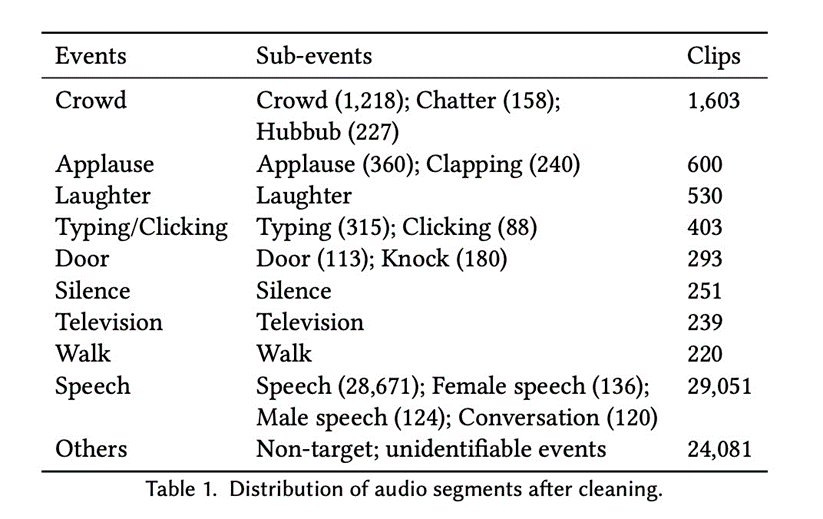
\includegraphics[width=0.7\linewidth]{screenshot001}
	\caption{}
	\label{fig:screenshot001}
\end{figure}

%\section{Context}
%\section{Motivation}
%\section{Hypothesis}
%\section{Client}
%\section{Scope}
\section{Research Questions}

My research questions are:

How can a end-to-end human activity recognition system be built based on ambient audio sensing using mobile devices in a multi-task approach for an office environment?

Sub questions:

\begin{itemize}
	\item What are the current approaches and limitations in the field of activity recognition using acoustic audio?\\
	To answer this question we're going to look at the research.
	\item How can we use multi-task learning to improve acoustic event recognition?\\
	To answer this question we're going to look at the research and find the steps for multi-task learning, as well as check out any approaches that have been tried.
	\item How can a multi-task acoustic event detection system be developed for lifelog modeling in an office environment?\\
	To answer this question we're going to see how we adapt the system to the current dataset and the requirements for a lifelog, as well as try to leverage benefits from knowing it's for an office environment.
	\item How feasible is it to build a multi-task acoustic event classifier for mobile devices? \\
	To answer this question, we're going to build a multi-task classifier as well as a classifier for separate events, check the difference in performance, memory usage and evaluate its feasibility for mobile devices.
\end{itemize}


%\section{Challenges}

%According to \cite{chandrakala2019environmental}, challenges/characteristics in correlation with the scenes:

%\begin{itemize}
%	\item Signal-to-noise ratio (SNR) is typically very small in an audio signal, particularly if the microphone is not very near to the acoustic source (Crocco et al. 2016)
%	\item Discriminative information exists in low-frequency ranges (chachada and Kuo 2014)
%	\item environmental sounds/scenes do not have any specific structures such as phonemes or prosody (Cowling and Sitte 2003).
%\end{itemize}

%Challenges in connection to automatic recognition of audio scenes or events:

%\begin{itemize}
%	\item Recognizing many events from a single environment, such as an office room, a residential area, or a busy street that may have multiple sound sources (Messaros et al. 2010, 2015)
%	\item A dictionary of basic units is unidentifiable (Cowling and Sitte 2003)
%	\item the existence of overlapping or polyphonic events (Gemmeke et al. 2013; Mesaros et al. 2010)
%	\item recognition of confusing scenes e.g. street traffic vs. restaurant (Ntalampiras et al. 2011)
%	\item Lack of discrimination among scenes such as pedestrian street market, quiet street and shop (Rakotomamonjy and Gasso 2015)
%	\item identifying acoustic sound sources in the presence of background noise (Beltran et al. 2015; Salamon et al. 2014)
%	\item The existence of certain audio events in multiple environments, e.g., "gunshot" sound present in environments such as street and home (Heittola et al. 2013)
%	\item The multimodal surveillance systemn for critical indoor environments (Moeslund et al. 2014)
%	\item lack of standard and multimodal datasets (Chchada and Kuo 2013);
%	\item Lack of robust and compact representation learning techniques for audio scenes and sound events. (Ozer et al. 2018; Phan et al. 2017)
%\end{itemize}



\section{Contributions}

My contributions are:

\begin{itemize}
	\item A systematic literature review of the state-of-the-art deep learning approaches in Acoustic Sound Detection (AED) as well as Deep learning multi-Task learning algorithms, as well as investigating the design space for use in lifelogging systems.
	\item A neural network-based multi-task system able to detect and classify multiple overlapping events in audio fragments.
	\item Application and analysis of this classifier on a specific use-case, namely an office environment.
	\item Evaluation of the feasibility to run single and multi-task classifiers on mobile devices. 
\end{itemize}
\section{Outline}






	
	% fix this
	% fix questions
	
%	\chapter{Research Goal}
	In this thesis different combinations of tasks are evaluated in a MTL setup. The example of (2017 Bingel and Sogaard. Identifying beneficial task relations for multi-task learning in deep neural networks) is followed in that this work will try to identify data characterstics and patterns both in single-task and dual-task learning that predict task interactions in MTL deep neural networks. 
	
	\begin{table}[ht]
		\caption{Research questions} % title of Table
		\centering % used for centering table
		\begin{tabular}{p{\textwidth}} % centered columns (4 columns)
			\hline\hline %inserts double horizontal lines
			Question \\ [0.5ex] % inserts table
			%heading
			\hline % inserts single horizontal line
			When do Acoustic Classification tasks learned in a deep learning multi-task hard parameter sharing set-up improve each other? \\ % inserting body of the table
			What dataset measurements are predictive of multi-task success? \\
			What single inference task measurements are predictive of multi-task success? \\
			When do multiple tasks learned simultaneously not decrease each other’s performance? \\ [1ex] % [1ex] adds vertical space
			\hline %inserts single line
		\end{tabular}
		\label{table:questions} % is used to refer this table in the text
	\end{table}

	
	\chapter{Research goal}
	In this thesis different combinations of tasks are evaluated in a MTL setup. The example of (2017 Bingel and Sogaard. Identifying beneficial task relations for multi-task learning in deep neural networks) is followed in that this work will try to identify data characterstics and patterns both in single-task and dual-task learning that predict task interactions in MTL deep neural networks. 
	
	\begin{table}[ht]
		\caption{Research questions} % title of Table
		\centering % used for centering table
		\begin{tabular}{p{\textwidth}} % centered columns (4 columns)
			\hline\hline %inserts double horizontal lines
			Question \\ [0.5ex] % inserts table
			%heading
			\hline % inserts single horizontal line
			When do Acoustic Classification tasks learned in a deep learning multi-task hard parameter sharing set-up improve each other? \\ % inserting body of the table
			
			\hline\hline %inserts double horizontal lines
			Subquestions \\ [0.5ex] % inserts table
			%heading
			\hline % inserts single horizontal line
			
			\\ [1ex] % [1ex] adds vertical space
			\hline %inserts single line
		\end{tabular}
		\label{table:questions} % is used to refer this table in the text
	\end{table}
	
	
	\chapter{Method}
	% \section{Experiment 1}
	
	\textbf{Research Question:} When do Acoustic Classification tasks, learned in a deep learning multi-task, hard parameter sharing set-up, improve each other? 
	\textbf{Research Method:} Implement different multi-class acoustic classification tasks from different corpi and different domains as well as simpler auxiliary tasks specifically aimed at improving performance of the main task. The classification model will be a DNN without any adjustments for any specific task, to generalize the observations for task interaction in a multi-task learning setting. Different measurements are taken from the datasets beforehand. Each task is run in a single task set up, with different measurements being kept from the learning process and results. The goal of the investigation is to assess whether improved performance for one of the tasks in a dual task learning set-up can be predicted from the dataset and single inference task measurements through regression analysis.\\
	
	\textbf{Task choice:}\\
	
	Main Tasks\\
	
%	-- EXPLANATIONS OF TASKS\\
	\begin{itemize}
		\item General Acoustic Event Detection: Acoustic event detection or Sound event detection refers to the task of locating and classifying Sound Events in an audio from real life environments. General purpose AED means no specific optim
		\item Acoustic Scene Classification: Acoustic Scene Classification involves the automatic detection of the environment in an audio stream. Both indoor as well as outdoor environments can be included, with the length duration of a scene being long.
		\item Speaker Identification is the task of identifying the person speaking in an audio clip.
		\item Keyword Spotting aims at detecting predefined keywords in audio streams.
		\item Environmental Sound Classification (KEEP THIS FOR OTHER EXPERIMENT WHERE YOU INVESTIGATE DIFFERENT AED SETUPS like keeping out speech, polyphonic and monophonic, different datasets, specific vs non specific environment)
	\end{itemize}

%	-- REASONS WHY FOR THESE TASKS (use in other and general interest)\\
%	- Georgiev used them\\
%	- Most interesting for lifelogging purposes according to gurrin\\
%	- Different and multiple domains\\
%	- Domains: Speech, Environment, Music\\
%	- Different and multiple corpuses\\

	
	These are the main tasks, chosen to represent a variety of audio sensing tasks in the research. The tasks are more often then not the primary focus in audio sensing research, and are more complex in nature, with a multi-class classification goal. The choice was made for this specific set of tasks for multiple reasons. First of all, Gurrin et al. identified the main interests for audio sensing tasks for lifelogging purposes as being the identification of activities, audio events, location, people and keywords in dialogue, each of which is represented as a main task here. Futhermore, in work done by Georgiev, a system is built which combined Acoustic Scene Classification, Speaker Identification, Emotion Recognition and Stress detection, finding that all could be combined in a single multi-task DNN set-up without significant performance decrease. In this work the same DNN structure will as it has shown to perform well on multiple audio sensing tasks as well as allow direct verification for its findings. Furthermore are all (main and auxiliary) tasks chosen so that they would span multiple domains (Speech, Environment and Music), as well as multiple different datasets. 


	Auxiliary Tasks\\
	
	\begin{itemize}
		\item Music/Speech Detection
		\item Voice Activity Detection
		\item Emotion Detection
		\item Gender Detection
		\item Audio Tagging
		\item Event Activity Detection
		\item Stress Detection
		\item Music Instrument detection
	\end{itemize}
	
	
	%-- WHAT ARE AUXILIARY TASKS\\
	%- Smaller label set, simpler task\\
	%- Used to improve performance in other task\\
	%-- REASONS WHY FOR THESE TASKS (use in other and general interest)\\
	%- Used in literature\\
	%- M/S, Event activity detection and VAD used to explicitly learn how to differentiate between what is in the audio\\
	%- Emotion detection, stress detection and gender detection as semantic detection in speech domain, demonstrate whether it improves speech detection in other tasks, as well as performance of tasks in speech domain\\
%	- Music Instrument detection same as previous but for music domain\\
%	- Audio Tagging as a different specificity level compared to general audio event detection\\
%	-- REFER TO USE IN PAPERS\\
	
	The previous mentioned main tasks are supplemented by a list of auxiliary tasks, which are generally simpler tasks that are not often the main research goal but added as a side task to explicitly improve the main task. They often can be performed on the same dataset as the main task. Each task is treated as a main task and combined with all the other tasks. These are still mentioned as separate, as they are explicitly chosen for a specific relationship with at least one of the main tasks. Some tasks - e.g. Emotion detection - are also only considered auxiliary tasks in this context therefore. \\
	
	The reason for each inclusion will be disclosed next. There are three main categories the reasons of inclusion fall in, which relation to the main tasks this work aims to investigate: Simple differentiation, semantic detection in a specific domain and different specificity level. 
	
	\begin{itemize}
		\item With simple differentiation, the Music/Speech detection, Voice Activity Detection and Event Activity Detection tasks fall under this. These tasks simply try to differentiate if activity of a certain type is or isn't happening at a certain point. The hypothesis is that simple differentiation helps to build a representation that would make less errors for tasks where wrongfully differentiating the target labels of these tasks leads to prediction errors in its own results. 
		\begin{itemize}
			\item Music/Speech Detection: The task of classifying audio in a stream between Music, Speech or neither. This is included as it learns to differentiate between different domains which might be beneficial for all (main) tasks
			\item Voice Activity Detection: The task of detecting voice activity in a stream. This learns a representation that can differentiate specifically between what sound is or is not coming from a voice, which might lower the number of classification errors happening in SI and KS when the sound is not a voice, as well as AED for discriminating the speech label.
			\item Event Activity Detection: The task of detecting whether or not a sound event is happening at a certain point. In the literature (REFERENCE) AED has often been defined as a multi-task problem, by splitting the tasks of detecting an event and determining the type of event (Audio Tagging) in two, while still learning them simultaneously and combining the results afterwards. This has lead to better performance to baseline single task AED systems. This inclusion might be beneficial for lowering detection errors when no (target) sound event is present AED, SI and KS. 
		\end{itemize}
	
		\item Next is semantic detection, which here means the Emotion detection, stress detection, gender detection in the speech domain and music instrument detection in the music domain. These try to identify a certain property of events in the audio. The idea of including this is to check whether identifying more complex properties of speech and music having a less direct link to the purposes of the main tasks can be beneficial for performance.
		\begin{itemize}
			\item Emotion Detection: The task of detecting emotion from speech and music. This was included in the work done by Georgiev as well as others. Emotion Detection is not expected to have any direct link to any of the main tasks, except perhaps a loose one with the speech domain tasks. 
			\item Gender Detection: The task of detecting gender of a speaker. This is directly linked to speaker identification, as the same speaker will have the same gender. 
			\item  Stress Detection: The task of detecting stress in speech audio. This was also included in the work done by Georgiev. Stress detection has a loose connection with the speech domain, but a direct one with Emotion Detection. It has a smaller target labelset size than Emotion Detection, in which we are interested due to previous observations that tasks with smaller target label sets make for better auxiliary tasks.
			\item  Music Instrument detection: The task of detecting which music instrument is played in an audio clip. This has a loose connection with the music domain, which might be interesting for better detection of music audio, leading to less wrongful labels for events that are out of target for the main tasks.
		\end{itemize}
	
		\item The last one is different specificity level, under which only audio tagging falls directly, as it is a simpler version of AED (you only need to identify what is happening in the whole clip and not when it is or is not present). The first category can be seen as a more specific subset of this with a small target label set though. The interest for this class is different, in the sense that it is more about reporting the difference adding a simplified version of the same task makes as well as comparing its interaction with the other tasks to the specific version.
		\begin{itemize}
			\item Audio Tagging: In AED research, improved results have been achieved by defining the task of AED as two separate tasks, namely Audio Tagging and Event Activity Detection, learned simultaneously in a multi-task framework. Besides this, work done by Huang et al. achieved the best results in the 2019 AED challenge by adding additional branches of audio tagging tasks (with different pooling methods) besides the main Audio Tagging/Event Detection branch. Therefore the interest lies in its comparison with the performance compared to single task AED as well as its interaction with other tasks in a multi-task framework.
		\end{itemize}
	\end{itemize}
	
	\begin{table}[ht]
		\caption{Tried Combinations} % title of Table
		\centering % used for centering table
		\begin{tabular}{p{0.2\textwidth}p{0.6\textwidth}p{0.2\textwidth}} % centered columns (4 columns)
			\hline\hline %inserts double horizontal lines
			Title & Tasks & Classifier   \\ [0.5ex] % inserts table
			%heading
			\hline % inserts single horizontal line
			\citet{lu2004multitask} & Automatic Speech Recognition; Speech Enhancement; Gender Detection & RNN \\ \hline
			\citet{panchapagesan2016multi} & Keyword Spotting; Large Vocabulary Continuous Speech Recognition Senones Targets Recognition & \\ \hline
			\citet{sakti2016deep} & Automatic Speech Recognition; Acoustic Event Detection & DNN \\ \hline
			\citet{georgiev2017heterogeneous} \citet{georgiev2017low} & Speaker Identification; Emotion Detection; Stress Detection; Acoustic Scene Classification & DNN \\ \hline
			\citet{kim2017speech} & Emotion Detection; Auxiliary tasks: Arousal Level; Valence Level; Gender Detection & CNN \\ \hline
			\citet{nwe2017convolutional} & Acoustic Scene Classification (Grouped scenes as different tasks) & \\ \hline
			\citet{sun2017compressed} & Keyword Spotting; Large Vocabulary Continuous Speech Recognition Phone Targets Recognition & \\ \hline
			\citet{kremer2018inductive} & Word Error Rate and Character-Level Automatic Speech Recognition & CNN \\ \hline
			\citet{morfi2018deep} & Audio Tagging; Event Activity Detection & DNN \\ \hline
			\citet{lee2019label} & Main Tasks: Audio Tagging; Speaker Identification; Speech Command Recognition (Keyword Spotting); Auxiliary Tasks: Next-Step prediction; Noise Reduction; Upsampling &  \\ \hline
			\citet{lopez2019keyword} & Keyword Spotting; Own-voice/External Speaker Detection & \\ \hline
			\citet{pankajakshan2019polyphonic} & Sound Activity Detection (Event Activity Detection); Sound Event Detection (Audio Tagging) & CRNN \\ \hline
			\citet{tonami2019joint} & Acoustic Event Detection; Acoustic Scene Classification & CRNN for AED, CNN for ASC  \\ \hline
		\end{tabular}
		\label{table:combinations} % is used to refer this table in the text
	\end{table}

	\begin{table}[ht]
		\caption{Tried Combinations (Continued)} % title of Table
		\centering % used for centering table
		\begin{tabular}{p{0.2\textwidth}p{0.6\textwidth}p{0.2\textwidth}} % centered columns (4 columns)
			\hline\hline %inserts double horizontal lines
			Title & Tasks & Classifier   \\ [0.5ex] % inserts table
			%heading
			\hline % inserts single horizontal line
			\citet{xia2019multi} & Acoustic Event Type Detection (Audio Tagging); Predict frame position information (Event Activity Detection) & CNN \\ \hline
			\citet{xu2019multi} & Acoustic Event Detection; Acoustic Scene Classification & \\ \hline
			\citet{zeng2019spectrogram} (1) & Emotion Detection; Music/Speech Classification & DNN \\ \hline
			\citet{zeng2019spectrogram} (2) & Accent Recognition; Speaker Identification & DNN \\ \hline
			\citet{abrol2020learning} & Fine and Coarse Labels Acoustic Scene Classification & DNN \\ \hline
			\citet{deshmukh2020multi} & Acoustic Event Detection; Reconstruct Time Frequency Representation of Audio &  CNN \\ \hline
			\citet{fernando2020temporarily} & Acoustic Event Type Detection (Audio Tagging); Predict Frame Position Information (Event Activity Detection) & LSTM \\ \hline
			\citet{huang2020guided} & Audio Tagging; Temporal Detection (Event Activity Detection) & CNN PT/PS model \\ \hline
			\citet{huang2020multi} & Audio Tagging; Event Boundary Detection (Event Activity Detection) & CNN \\ \hline
			\citet{tagliasacchi2020multi} & Keyword Spotting; Speaker Identification; Language Identification; Music/Speech Classification; Bird Audio Detection; Urban Acoustic Scene Classification; Music Instrument Pitch Detection; Music Instrument Detection & CNN  \\ \hline
			\citet{wu2020domain} & Keyword Spotting; Domain Prediction & \\
			[1ex] % [1ex] adds vertical space
			\hline %inserts single line
		\end{tabular}
		\label{table:combinations2} % is used to refer this table in the text
	\end{table}


	% This might be a different research question:
	% - How does splitting up AED in EAD and AT tasks affect the multi-task set-up?
	% - How does a general AED into different set-ups affect the multi-task set-up?

	% \textbf{Literature Observations:}\\
	
	
	\textbf{Neural Network:}\\
	%-- REFER TO GEORGIEV'S USE AND NLP RESEARCH JUSTIFICATION FOR USING 1\\
	
	\begin{figure}
		\centering
		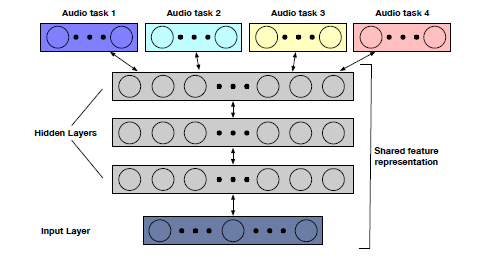
\includegraphics[width=0.9\linewidth]{NN.PNG}
		\caption{Multi-task DNN model}
		\label{fig:NN}
	\end{figure}

	%Basis: DNN feed-forward propagation classifier
	%Input: Statistical summaries of log filter banks
	%Architecture: Input and hidden layers are shared across potential combinations of audio analysis tasks -> Universal feature transformation that captures acoustic observations. 3 hidden layers with either 128, 256 or 512 nodes each, hard parameter sharing. Soft-max layer at the task-specific layers, updated separately depending on the training input instance.
	%Training: mini-batch stochastic gradient descent all audio tasks simultaneously
	%Fine-tuning: backpropagation
	%Additional: Keep the hyper-parameters fixed across single-task and multi-task settings for comparison. Use fixed random seed set upfront to facilitate replicability. Do not use any task-specific features or pre-trained embeddings for initialisation to delimit the behaviour of the architecture and analyse the interaction between tasks.
	
	The architecture is based on the system, described by \citet{georgiev2017heterogeneous}, which is a Deep Neural Network (DNN) feed-forward propagation classifier. As seen in figure \ref{fig:NN}, in a multi-task setting, all tasks share the same input and hidden layers, with task-specific output layers. This leads to these layers being used as a universal feature transformation which captures acoustic observations from different tasks. For the input, features have to be extracted from the audio. In the original work this is implemented by statistical summaries of log filter banks, extracted from each audio frame. They use summaries both for reducing the input feature complexity as well as allowing a representation of the same size across multiple tasks. \\
	
	To allow for comparison and analysis of the interaction between tasks, this work follows the approach from \cite{alonso2016multitask} and \cite{bingel2017identifying} the hyperparameters (this includes a fixed random seed set) and the architecture will be kept the same, regardless of which and the number of tasks learned. The set-up \citet{georgiev2017heterogeneous} had was 3 hidden layers which were tested at 128, 256 or 512 in each layer, with a soft-max pooling layer at the output layers. The output layers are updated separately depending on whether the training input instance is one for their own task. Furthermore, no task-specific features, nor any pre-trained embeddings will be used for initialisation to avoid any task bias. \\
	
	The training is done by mini-batch Stochastic Gradient Descent (SGD) on all audio tasks simultaneously, which is the key to succesfully training the multi-task DNN \citep{georgiev2017heterogeneous}. The samples are randomised across tasks before being fed into the DNN system. Backpropagation is then used for the fine-tuning of the DNN, which again only trains the softmax layer for the task at hand with the other softmax layers being kept intact. \\
	
	This set-up is chosen for the same reasons as Georgiev, namely due to the fact that it proved to be successful in multiple audio analysis tasks, as well as providing a good comparison opportunity for analysing the results. As \citet{bingel2017identifying} noted in their work as well however, the fixed hyper-parameters make the results only applicable to the scenario where one wants to know whether MTL works in the chosen parameter configuration.\\
	
	\textbf{Dataset measurements:}\\
	One way of structurally figuring out when multiple tasks can improve each other is described in \citet{alonso2016multitask} and \citet{bingel2017identifying}, where they try to predict which dataset and task features correlate to improvements in the multi-task setting for NLP tasks. \citet{bingel2017identifying} builds a regression analysis system for this to find the Pearson Coefficiënt between pre-measured data and the change in F1 score from single to multi-task systems. There are 3 groups of dataset measurements which will be examined: Dataset features, Information Theory derived features and Single task inference features. \\
	
	\textbf{Dataset features}
	\begin{itemize}
		\item Number of labels
		\item Number of clips
		\item Number of labeled frames
		\item Type/token ratio
		\item Labels per domain
		\item Dataset size
	\end{itemize}
	
	\textbf{Information Theory derived features}
	
	In \citet{alonso2016multitask}, these were found to be the most informative features. The interest is in determining whether these results are transferable to the audio domain.
	\begin{itemize}
		\item label entropy: Entropy of the label distribution
		\item label kurtosis: Indicates the skewness of a distribution
	\end{itemize}
	
	\textbf{Learning curve features}
	
	In \citet{bingel2017identifying} these were one of the most informative features. This involves taking measurements of the learning curve for the single tasks at different stages.
	\begin{itemize}
		\item Curve gradients: The gradients of the loss curve, taken at 10, 20, 30, 50 and 70 percent of the total number of batches
		\item Fitted log-curve: A logarithmic functio is fitted to the loss curve values, where the function is of the form L(i) = a*ln(c*i+d) + b where a and c are features that describe the steepness of the learning curve.
	\end{itemize}		
	
	\textbf{Audio features}
	
	Along with the features from the NLP research, additional audio related features are taken in account, which have been mentioned in the literature.
	\begin{itemize}
		\item Average sample length
		\item Total length of dataset (in seconds)
		\item Sampling rate
		\item Signal to Noise Ratio
	\end{itemize}
	
	\textbf{Non-numetric Factors}
	
	Finally there are also non-numetric Factors that might have an impact. 
	\begin{itemize}
		\item Overlapping\\Non-overlapping events
		\item Unlabeled, weakly labeled and strongly labeled dataset
		\item Mono or Stereo channel
	\end{itemize}
	
	\textbf{Evaluation:}\\
	
	The evaluation will 
	
	For evaluation these are the general metrics
	
	\begin{itemize}
		\item Averaged F1 score: The event categories are considered equally important \cite{phan2019unifying}
		\item Overall F1 score: The event instances are considered equally important \cite{phan2019unifying}
		\item Accuracy: Used in contexts where false positives and false negatives are less important than the rate of true positives and true negatives, which is often the case in audio sensing tasks.
		\item Detection Error Rate (ER): Used for evaluating correct segmentation of events from a continuous test signal \cite{phan2019unifying}
		\item Area Under the Receiver Operating Characteristic Curve (ROC AUC): plots the true positive rate against the false positive rate, with the metric being calculated from the area under the plot. Random guesses have an AUC of 0.5 \cite{deshmukh2020multi}
		\item Pearson coefficient: Measure for correlation between two variables. In this case, this will be the correlation of the numeric measurements from the dataset. For this a regression analysis system will be built.
		\item Intermediate output variances: Used in \cite{xia2019multi}  (to prove they can average respective noise patters, see 2020 Xia et al.)
		%\item Ablation Model of input embeddings to evaluate discriminative feature learning (see 2020 Fernando, 2020 Deshmukh et al.) different experiment
		%\item SNR (see 2016 Sakti et al.) Different experiment
		\item Efficiency: Combining tasks in a multi-task setting is used both for performance as efficiency purposes. Two metrics will be evaluated, following \cite{georgiev2017heterogeneous}. Both of these will be compared to running a single inference task and the combined time of running all combined tasks separately.
		\begin{itemize}
			\item Runtime: The time needed for performing audio classification 
			\item Memory: The size of the trained multi-task DNN compared to the single task and combined single tasks variants.
		\end{itemize}
	\end{itemize}

	Lastly, this work will take a look at class relationships in the context of multi-task. In the research, a few observations have already been made, in regards to the effect of the combination of tasks on certain classes. Specifically in this experiment, two effects will be specifically investigated. 
	
	\begin{itemize}
		\item \textbf{Speech related tasks for AED}: (REFERENCE) multiple observations have been made that for a general AED classifier, the Speech class is often mislabeled and causes mislabels of events like coughs. (CITE) notes that this is due to the fact that speech signals and environmental audio signals have a different structure. Therefore, this experiment especially interested in whether and/or which tasks in the speech domain can improve the speech class detection in AED. 
		\item \textbf{AED events only happening in certain scenes for ASC}: (REFERENCE) has noticed, when combining AED and ASC that AED can improve ASC, especially when certain events only happen in specific scenes. This was also found to go in the other direction, namely that events happening in multiple scenes will lead to a worse performance in ASC. This means the overview will be made of which events are in which scenes and also which ones are unique. 
	\end{itemize}

	
	% streamline experiments define in the beginning
	% revisit literature
	% start each experiment reviewing literature
	% next meeting: done with the first exp
	% give presentation
	% allows them to assist
	
	\section{Experiment 1}
	
	\textbf{Research Question:} When do unrelated Acoustic Classification tasks, learned in a deep learning multi-task, hard parameter sharing set-up, improve each other? \\
	\textbf{Research Method:} Implement different multi-class acoustic classification tasks from different corpi and different domains. The classification model will be a DNN without any adjustments for any specific task, to generalize the observations for task interaction in a multi-task learning setting. Different measurements are taken from the datasets beforehand. Each task is run in a single task set up, with different measurements being kept from the learning process and results. The goal of the investigation is to assess whether improved performance for one of the tasks in a dual task learning set-up can be achieved, or to which degree these tasks can be combined without a significant performance decrease for efficiency purposes.\\
	
	\textbf{Task choice:}\\
	
	Main Tasks\\
	
%	-- EXPLANATIONS OF TASKS\\
	\begin{itemize}
		\item General Acoustic Event Detection: Acoustic event detection or Sound event detection refers to the task of locating and classifying Sound Events in an audio from real life environments. General purpose AED means no specific optim
		\item Acoustic Scene Classification: Acoustic Scene Classification involves the automatic detection of the environment in an audio stream. Both indoor as well as outdoor environments can be included, with the length duration of a scene being long.
		\item Speaker Identification is the task of identifying the person speaking in an audio clip.
		\item Keyword Spotting aims at detecting predefined keywords in audio streams.
	\end{itemize}

%	-- REASONS WHY FOR THESE TASKS (use in other and general interest)\\
%	- Georgiev used them\\
%	- Most interesting for lifelogging purposes according to gurrin\\
%	- Different and multiple domains\\
%	- Domains: Speech, Environment, Music\\
%	- Different and multiple corpuses\\

	
	These are the main tasks, chosen to represent a variety of audio sensing tasks in the research. The tasks are more often then not the primary focus in audio sensing research, and are more complex in nature, with a multi-class classification goal. The choice was made for this specific set of tasks for multiple reasons. First of all, Gurrin et al. identified the main interests for audio sensing tasks for lifelogging purposes as being the identification of activities, audio events, location, people and keywords in dialogue, each of which is represented as a main task here. Futhermore, in work done by Georgiev, a system is built which combined Acoustic Scene Classification, Speaker Identification, Emotion Recognition and Stress detection, finding that all could be combined in a single multi-task DNN set-up without significant performance decrease. In this work the same DNN structure will as it has shown to perform well on multiple audio sensing tasks as well as allow direct verification for its findings. Furthermore are all (main and auxiliary) tasks chosen so that they would span multiple domains (Speech, Environment and Music), as well as multiple different datasets. \\

	
	\textbf{Neural Network:}\\
	%-- REFER TO GEORGIEV'S USE AND NLP RESEARCH JUSTIFICATION FOR USING 1\\
	
	\begin{figure}
		\centering
		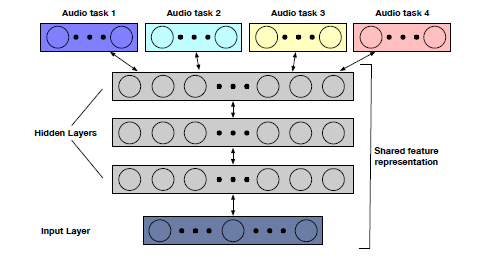
\includegraphics[width=0.9\linewidth]{NN.PNG}
		\caption{Multi-task DNN model}
		\label{fig:NN}
	\end{figure}

	%Basis: DNN feed-forward propagation classifier
	%Input: Statistical summaries of log filter banks
	%Architecture: Input and hidden layers are shared across potential combinations of audio analysis tasks -> Universal feature transformation that captures acoustic observations. 3 hidden layers with either 128, 256 or 512 nodes each, hard parameter sharing. Soft-max layer at the task-specific layers, updated separately depending on the training input instance.
	%Training: mini-batch stochastic gradient descent all audio tasks simultaneously
	%Fine-tuning: backpropagation
	%Additional: Keep the hyper-parameters fixed across single-task and multi-task settings for comparison. Use fixed random seed set upfront to facilitate replicability. Do not use any task-specific features or pre-trained embeddings for initialisation to delimit the behaviour of the architecture and analyse the interaction between tasks.
	
	The architecture is based on the system, described by \citet{georgiev2017heterogeneous}, which is a Deep Neural Network (DNN) feed-forward propagation classifier. As seen in figure \ref{fig:NN}, in a multi-task setting, all tasks share the same input and hidden layers, with task-specific output layers. This leads to these layers being used as a universal feature transformation which captures acoustic observations from different tasks. For the input, features have to be extracted from the audio. In the original work this is implemented by statistical summaries of log filter banks, extracted from each audio frame. They use summaries both for reducing the input feature complexity as well as allowing a representation of the same size across multiple tasks. \\
	
	To allow for comparison and analysis of the interaction between tasks, this work follows the approach from \cite{alonso2016multitask} and \cite{bingel2017identifying} the hyperparameters (this includes a fixed random seed set) and the architecture will be kept the same, regardless of which and the number of tasks learned. The set-up \citet{georgiev2017heterogeneous} had was 3 hidden layers which were tested at 128, 256 or 512 in each layer, with a soft-max pooling layer at the output layers. The output layers are updated separately depending on whether the training input instance is one for their own task. Furthermore, no task-specific features, nor any pre-trained embeddings will be used for initialisation to avoid any task bias. \\
	
	The training is done by mini-batch Stochastic Gradient Descent (SGD) on all audio tasks simultaneously, which is the key to succesfully training the multi-task DNN \citep{georgiev2017heterogeneous}. The samples are randomised across tasks before being fed into the DNN system. Backpropagation is then used for the fine-tuning of the DNN, which again only trains the softmax layer for the task at hand with the other softmax layers being kept intact. \\
	
	This set-up is chosen for the same reasons as Georgiev, namely due to the fact that it proved to be successful in multiple audio analysis tasks, as well as providing a good comparison opportunity for analysing the results. As \citet{bingel2017identifying} noted in their work as well however, the fixed hyper-parameters make the results only applicable to the scenario where one wants to know whether MTL works in the chosen parameter configuration.\\
	
	\textbf{Dataset measurements:}\\
	One way of structurally figuring out when multiple tasks can improve each other is described in \citet{alonso2016multitask} and \citet{bingel2017identifying}, where they try to predict which dataset and task features correlate to improvements in the multi-task setting for NLP tasks. \citet{bingel2017identifying} builds a regression analysis system for this to find the Pearson Coefficiënt between pre-measured data and the change in F1 score from single to multi-task systems. There are 3 groups of dataset measurements which will be examined: Dataset features, Information Theory derived features and Single task inference features. \\
	
	\textbf{Dataset features}
	\begin{itemize}
		\item Number of labels
		\item Number of clips
		\item Number of labeled frames
		\item Type/token ratio
		\item Labels per domain
		\item Dataset size
	\end{itemize}
	
	\textbf{Information Theory derived features}
	
	In \citet{alonso2016multitask}, these were found to be the most informative features. The interest is in determining whether these results are transferable to the audio domain.
	\begin{itemize}
		\item label entropy: Entropy of the label distribution
		\item label kurtosis: Indicates the skewness of a distribution
	\end{itemize}
	
	\textbf{Learning curve features}
	
	In \citet{bingel2017identifying} these were one of the most informative features. This involves taking measurements of the learning curve for the single tasks at different stages.
	\begin{itemize}
		\item Curve gradients: The gradients of the loss curve, taken at 10, 20, 30, 50 and 70 percent of the total number of batches
		\item Fitted log-curve: A logarithmic functio is fitted to the loss curve values, where the function is of the form L(i) = a*ln(c*i+d) + b where a and c are features that describe the steepness of the learning curve.
	\end{itemize}		
	
	\textbf{Audio features}
	
	Along with the features from the NLP research, additional audio related features are taken in account, which have been mentioned in the literature.
	\begin{itemize}
		\item Average sample length
		\item Total length of dataset (in seconds)
		\item Sampling rate
		\item Signal to Noise Ratio
	\end{itemize}
	
	\textbf{Non-numetric Factors}
	
	Finally there are also non-numetric Factors that might have an impact. 
	\begin{itemize}
		\item Overlapping\\Non-overlapping events
		\item Unlabeled, weakly labeled and strongly labeled dataset
		\item Mono or Stereo channel
	\end{itemize}
	
	\textbf{Evaluation:}\\
	
	The evaluation will 
	
	For evaluation these are the general metrics
	
	\begin{itemize}
		\item Averaged F1 score: The event categories are considered equally important \cite{phan2019unifying}
		\item Overall F1 score: The event instances are considered equally important \cite{phan2019unifying}
		\item Accuracy: Used in contexts where false positives and false negatives are less important than the rate of true positives and true negatives, which is often the case in audio sensing tasks.
		\item Detection Error Rate (ER): Used for evaluating correct segmentation of events from a continuous test signal \cite{phan2019unifying}
		\item Area Under the Receiver Operating Characteristic Curve (ROC AUC): plots the true positive rate against the false positive rate, with the metric being calculated from the area under the plot. Random guesses have an AUC of 0.5 \cite{deshmukh2020multi}
		\item Intermediate output variances: Used in \cite{xia2019multi} to prove they can average respective noise patters
		\item Efficiency: Combining tasks in a multi-task setting is used both for performance as efficiency purposes. Two metrics will be evaluated, following \cite{georgiev2017heterogeneous}. Both of these will be compared to running a single inference task and the combined time of running all combined tasks separately.
		\begin{itemize}
			\item Runtime: The time needed for performing audio classification 
			\item Memory: The size of the trained multi-task DNN compared to the single task and combined single tasks variants.
		\end{itemize}
	\end{itemize}

	Lastly, this work will take a look at class relationships in the context of multi-task. In the research, a few observations have already been made, in regards to the effect of the combination of tasks on certain classes. Specifically in this experiment, two effects will be specifically investigated. 
	
	\begin{itemize}
		\item \textbf{Speech related tasks for AED}: (REFERENCE) multiple observations have been made that for a general AED classifier, the Speech class is often mislabeled and causes mislabels of events like coughs. (CITE) notes that this is due to the fact that speech signals and environmental audio signals have a different structure. Therefore, this experiment especially interested in whether and/or which tasks in the speech domain can improve the speech class detection in AED. 
		\item \textbf{AED events only happening in certain scenes for ASC}: (REFERENCE) has noticed, when combining AED and ASC that AED can improve ASC, especially when certain events only happen in specific scenes. This was also found to go in the other direction, namely that events happening in multiple scenes will lead to a worse performance in ASC. This means the overview will be made of which events are in which scenes and also which ones are unique. 
	\end{itemize}

	\section{Experiment 2}

\textbf{Research Question:} What measurements can predict success in the multi-task set-up? \\

\textbf{Research Method:} Build a regression analysis system to compute the pearson correlation between the dataset and single task measurements and the multi-task performance shift. The goal of the investigation is to assess whether improved performance for one of the tasks in a dual task learning set-up can be predicted from the dataset and single inference task measurements through regression analysis.\\

\textbf{Dataset measurements:}\\
The dataset and single task measurements are described in Experiment 1 (except for the non-numetric factors). The same structure as \citet{bingel2017identifying} will be used for the regression as it is a good evaluation template, as well as making it possible to compare whether similar measurements are good predictors between NLP and Audio tasks. \\

\textbf{Regression Analysis} \\



\textbf{Evaluation:}\\

Any consistency in measurements that are good predictors for multi-task success between tasks will be looked for. The logistic regression will take the binarized results of the micro-averaged F1 scores from Experiment 1 (and the results from subsequent experiments) and be used to predict the benefits or detriments of MTL setups based on the computed features. An observation from the NLP research to verify is that multi-task gains seemed to be more likely for main tasks that quickly plateau with non-plateauing tasks, which might hold for audio tasks. \citet{bingel2017identifying} uses the mean performance of 100 runs of randomized five-fold cross-validation.

\begin{itemize}
	\item Pearson coefficient: Measure for correlation between two variables. In this case, this will be the correlation of the numeric measurements from the dataset. For this a regression analysis system will be built.
\end{itemize}

	\section{Experiment 3}
	
	\textbf{Research Question:} 
	Can auxiliary tasks be added to the multi-task set-up, to improve classification performance of (certain) main tasks? \\
	
	\textbf{Research Method:} Implement different auxiliary tasks specifically aimed at improving performance of one or more main tasks. The classification model will be the same DNN without any extra adjustments. The auxiliary tasks are chosen from the multi-task audio sensing literature, where they have proven to show positive results when combined with one of the main tasks. The aim is to find whether and which results are somewhat replicable in the current set-up, as well as again figuring out which factors can be related to positive improvements. All auxiliary tasks will be treated as main tasks in this experiment, in the sense that they will also be tested in combination with each other without any main task necessarily being present.\\
	
	\textbf{Task choice:}\\
	
	Auxiliary Tasks\\
	
	\begin{itemize}
		\item Music/Speech Detection
		\item Voice Activity Detection
		\item Emotion Detection
		\item Gender Detection
		\item Audio Tagging
		\item Event Activity Detection
		\item Stress Detection
		\item Music Instrument detection
	\end{itemize}
	
	
	%-- WHAT ARE AUXILIARY TASKS\\
	%- Smaller label set, simpler task\\
	%- Used to improve performance in other task\\
	%-- REASONS WHY FOR THESE TASKS (use in other and general interest)\\
	%- Used in literature\\
	%- M/S, Event activity detection and VAD used to explicitly learn how to differentiate between what is in the audio\\
	%- Emotion detection, stress detection and gender detection as semantic detection in speech domain, demonstrate whether it improves speech detection in other tasks, as well as performance of tasks in speech domain\\
%	- Music Instrument detection same as previous but for music domain\\
%	- Audio Tagging as a different specificity level compared to general audio event detection\\
%	-- REFER TO USE IN PAPERS\\
	
	The previous mentioned main tasks are supplemented by a list of auxiliary tasks, which are generally simpler tasks that are not often the main research goal but added as a side task to explicitly improve the main task. They often can be performed on the same dataset as the main task. Each task is treated as a main task and combined with all the other tasks. These are still mentioned as separate, as they are explicitly chosen for a specific relationship with at least one of the main tasks. Some tasks - e.g. Emotion detection - are also only considered auxiliary tasks in this context therefore. \\
	
	The reason for each inclusion will be disclosed next. There are three main categories the reasons of inclusion fall in, which relation to the main tasks this work aims to investigate: Simple differentiation, semantic detection in a specific domain and different specificity level. 
	
	\begin{itemize}
		\item With simple differentiation, the Music/Speech detection, Voice Activity Detection and Event Activity Detection tasks fall under this. These tasks simply try to differentiate if activity of a certain type is or isn't happening at a certain point. The hypothesis is that simple differentiation helps to build a representation that would make less errors for tasks where wrongfully differentiating the target labels of these tasks leads to prediction errors in its own results. 
		\begin{itemize}
			\item Music/Speech Detection: The task of classifying audio in a stream between Music, Speech or neither. This is included as it learns to differentiate between different domains which might be beneficial for all (main) tasks
			\item Voice Activity Detection: The task of detecting voice activity in a stream. This learns a representation that can differentiate specifically between what sound is or is not coming from a voice, which might lower the number of classification errors happening in SI and KS when the sound is not a voice, as well as AED for discriminating the speech label.
			\item Event Activity Detection: The task of detecting whether or not a sound event is happening at a certain point. In the literature (REFERENCE) AED has often been defined as a multi-task problem, by splitting the tasks of detecting an event and determining the type of event (Audio Tagging) in two, while still learning them simultaneously and combining the results afterwards. This has lead to better performance to baseline single task AED systems. This inclusion might be beneficial for lowering detection errors when no (target) sound event is present AED, SI and KS. 
		\end{itemize}
	
		\item Next is semantic detection, which here means the Emotion detection, stress detection, gender detection in the speech domain and music instrument detection in the music domain. These try to identify a certain property of events in the audio. The idea of including this is to check whether identifying more complex properties of speech and music having a less direct link to the purposes of the main tasks can be beneficial for performance.
		\begin{itemize}
			\item Emotion Detection: The task of detecting emotion from speech and music. This was included in the work done by Georgiev as well as others. Emotion Detection is not expected to have any direct link to any of the main tasks, except perhaps a loose one with the speech domain tasks. 
			\item Gender Detection: The task of detecting gender of a speaker. This is directly linked to speaker identification, as the same speaker will have the same gender. 
			\item  Stress Detection: The task of detecting stress in speech audio. This was also included in the work done by Georgiev. Stress detection has a loose connection with the speech domain, but a direct one with Emotion Detection. It has a smaller target labelset size than Emotion Detection, in which we are interested due to previous observations that tasks with smaller target label sets make for better auxiliary tasks.
			\item  Music Instrument detection: The task of detecting which music instrument is played in an audio clip. This has a loose connection with the music domain, which might be interesting for better detection of music audio, leading to less wrongful labels for events that are out of target for the main tasks.
		\end{itemize}
	
		\item The last one is different specificity level, under which only audio tagging falls directly, as it is a simpler version of AED (you only need to identify what is happening in the whole clip and not when it is or is not present). The first category can be seen as a more specific subset of this with a small target label set though. The interest for this class is different, in the sense that it is more about reporting the difference adding a simplified version of the same task makes as well as comparing its interaction with the other tasks to the specific version.
		\begin{itemize}
			\item Audio Tagging: In AED research, improved results have been achieved by defining the task of AED as two separate tasks, namely Audio Tagging and Event Activity Detection, learned simultaneously in a multi-task framework. Besides this, work done by Huang et al. achieved the best results in the 2019 AED challenge by adding additional branches of audio tagging tasks (with different pooling methods) besides the main Audio Tagging/Event Detection branch. Therefore the interest lies in its comparison with the performance compared to single task AED as well as its interaction with other tasks in a multi-task framework.
		\end{itemize}
	\end{itemize}
	


	% This might be a different research question:
	% - How does splitting up AED in EAD and AT tasks affect the multi-task set-up?
	% - How does a general AED into different set-ups affect the multi-task set-up?

	
	
	\textbf{Evaluation:}\\
	
	Aside from the Evaluation metrics described in the previous experiment, this will also include qualitative comparisons with results from the literature, including the difference in set-up, in order to evaluate how the difference in set-up affects multi-task performance.


	
	\section{Experiment 4}

% Same or different datasets
	\textbf{Research Question:} What is the effect of the choice of dataset in auxiliary tasks?\\
	
	\textbf{Research Method:} Implement and compare the performance of combining tasks when training on the same dataset as a main task, compared to using a different dataset. \\
	
	\textbf{Possible:} 
		
	\begin{itemize}
		\item AED \& ASC
		\item Speaker Identification \& Keyword detection (Kaggle2018)
		\item AED \& Music/Speech Detection (verify)
		\item AED \& Voice Activity Detection
		\item AED \& Audio Tagging
		\item AED \& Event Activity Detection
		\item (if AED and ASC contain the same classes in the combined subset, then everything above can be combined with ASC as well)
		\item Speaker Identification \& Music/Speech Detection (verify)
		\item Speaker Identification \& Voice Activity Detection (verify)
		\item Speaker Identification \& Emotion Detection (verify)
		\item Speaker Identification \& Gender Detection
		\item Speaker Identification \& Stress Detection (verify)
		\item Keyword Detection \&  Music/Speech Detection (verify)
		\item Keyword Detection \&  Voice Activity Detection
		\item Keyword Detection \&  Emotion Detection (verify)
		\item Keyword Detection \&  Gender Detection
		\item Keyword Detection \&  Event Activity Detection
		\item Keyword Detection \&  Stress Detection (verify)
	\end{itemize}
	\section{Experiment 5}

\textbf{Introduction}
In previous research, observations have been made that the multi-task setting is affected by the label overlap between classes. One example of this is in (REFERENCE), where they observe that, when combining AED and ASC, that the accuracy of the ASC task improved when an output label (i.e. a scene) did not share any output labels (i.e. sound events) with other scenes. When 2 scenes did share a number of sound events, the set-up had more difficulty differentiating the scenes correctly. In the same vein, it has been observed (REFERENCE) that including an Environmental Sound Classification task (i.e. AED task, but without speech-related labels) can improve speech domain tasks. This experiment will investigate the effect of keeping certain instances out of a task, compared to the case where the tasks have overlapping label relationships. \\

\textbf{Research Question:} How does class overlap affect combinations in the multi-task setting?\\

\textbf{Research Method:} Identify the task relationships in terms of overlap between labels and compare the results when training the network on a dataset where instances with these labels are left out.\\

	
	\chapter{Schedule}
	% Additional supervisor meetings
	% Clarifying what will be presented
	% Think about the kind of meetings and feedback
	% write down in an email indicating the week of the yesr = make it specific
	% ask specific date for meeting
	% send something if you expect feedback and what kind of feedback = part of the supervision schedule
	% first draft feedback when
	% send request for putting in the calendar end of this week or next week
	
	
	The first experiment will be about implementing and evaluating the main tasks and their combination in a multi-task setting.
	\begin{itemize}
		\item DNN classifier done 15/1
		\item Main task implementation done (4) 24/1
		\item Task inference experiments done 31/1
	\end{itemize}
	
	The second experiment
	\begin{itemize}
		\item done 14/2
	\end{itemize}
	
	The third experiment
	\begin{itemize}
		\item done 21/3
	\end{itemize}
	
	The fourth experiment
	\begin{itemize}
		\item done 11/4
	\end{itemize}

	The fifth experiment
	\begin{itemize}
		\item done 2/5
	\end{itemize}

	Finishing report done 30/5

	Done 
	
	% Extra experiments we should consider:
	% - the data input method variation (summary vs time sensitive features)
	
	
	
	
%	\chapter{Workplan}
%	
%	\section{Actions}
%	\begin{table}[ht]
%		\caption{Actions} % title of Table
%		\centering % used for centering table
%		\begin{tabular}{p{0.5\textwidth}p{0.5\textwidth}} % centered columns (4 columns)
%				\hline\hline %inserts double horizontal lines
%				Action & Question  \\ [0.5ex] % inserts table
%				%heading
%				\hline % inserts single horizontal line
%				Train and evaluate DNN on each task, take measurements of learning &  \\
%				Train and evaluate DNN on each task pair, take measurements of learning, compare to single task performance & Which tasks improve each other in a multi-task setting? \\
%				Build regression to predict duo performance from dataset and single inference task measurements & What dataset and single inference task measurements are predictive of multi-task success? \\
%				Train and evaluate DNN on each possible task combination, compareto single and duo task performance & Which tasks can be combined without a (significant) degration in performance? Can we predict multi-task success from single and dual inference tasks? \\
%				Build regression to predict multi performance from dataset and single inference task measurements & What dataset and single and dual inference task measurements are predictive of multi-task combinability? \\
%				Include a task which is the coarse grained version of another task & (Observation from the literature) Can a coarse grained version of a task improve the finer grained detection task? \\
%				Include tasks from the Speech, Music, Environment and general domain and observe their performance & What effect does the combining tasks with different domains have on performance in the multi-task setting? \\
%				Include a task that can be learned on a different or the same dataset as another & What is the effect of choosing the same or different dataset for a task in a multi-task setting? \\
%				Include a test where all the detectable classes in two tasks are correlated/uncorrelated with each other & Observation from the literature) Does a multi-task setting suffer when some classes in one task are completely correlated to classes in another? \\ [1ex] % [1ex] adds vertical space
%				\hline %inserts single line
%		\end{tabular}
%		\label{table:questions} % is used to refer this table in the text
%	\end{table}
%	
%	\begin{itemize}
%		\item Does using a task with more coarse grained labels as an aux task improve performance?
%		\item Does combining Speech/music/environmental domains lead to better results than only using a single domain? Can they be used to improve detection performance in certain classes?
%		\item Does learning an auxiliary to improve performance work better when performed on a different dataset or the same?
%		\item What is the effect of label conjecture?
%	\end{itemize}
%
	\begin{table}[ht]
		\caption{Datasets} % title of Table
		\centering % used for centering table
		\begin{tabular}{p{0.2\textwidth}p{0.3\textwidth}p{0.1\textwidth}p{0.3\textwidth}p{0.1\textwidth}} % centered columns (4 columns)
			\hline\hline %inserts double horizontal lines
			Tasks & Datasets & Count & Available & Count  \\ [0.5ex] % inserts table
			%heading
			\hline % inserts single horizontal line
			Acoustic Scene Classification & LITIS ROUEN; TUT Acoustic Scenes 2016 & 2 & TUT Acoustic Scenes 2016 & 1 \\
			Acoustic Event Detection & TUT SED 2016 for overlapping AED; DCASE 2020 Task 4; TUT Sound Events 2016; TUT Sound Events 2017; AudioSet adaptation & 5 & TUT SED 2016 for Overlapping AED; DCASE 2020 Task 4; AudioSet Adaptation & 3 \\
			Speaker Identification & Automatic Speaker Verification Spoofing and Counter measures challenge; LIBRISPEECH; Voice Cloning Toolkit; FSD Kaggle 2018; LibriAdapt & 5 & Automatic Speaker Verification Spoofing and Counter measures challenge; Librispeech; Voice Cloning Toolkit; FSD Kaggle 2018; LibriAdapt & 5 \\
			Keyword detection & TIMIT continuous speech corpus; FSD Kaggle 2018 & 2 & FSD Kaggle 2018 & 1 \\
			Music/Speech detection & Musan MUS dataset; RAVDESS & 2 & Musan MUS dataset; RAVDESS & 2 \\
			Voice Activity Detection & AMI Meeting; NIST OPEN SAT & 2 & AMI Meeting; & 1 \\
			Emotion Detection & Emotional Prosody Speech and Transcript Library; RAVDESS & 2 & RAVDESS & 1 \\
			Gender Detection & LibriAdapt & 1 & LibriAdapt & 1 \\
			Audio Tagging & DCASE 2020 Task 4; Urban SED; DCASE 2018 Task 4; FSD Kaggle 2018 & 4 & DCASE 2020 Task 4; Urban SED; FSD Kaggle 2018 & 3 \\ [1ex] % [1ex] adds vertical space
			\hline %inserts single line
		\end{tabular}
		\label{table:datasets} % is used to refer this table in the text
	\end{table}
%	
%	\section{Deep Learning Model}
%	A DNN will be made, sharing the same number of representations, with no task specific adjustments being made. The aim is to follow the model by Georgiev et al., both for comparing results as well as it being a good approach for multiple acoustic detection tasks.\\
%	
%	Afterwards logistic regression will be performed to determine the predictiveness of the performance results using the dataset and task inference measurements.\\
	
	\bibliographystyle{plainnat} 
	\bibliography{references}

\end{document}    